\section{Domain Analysis}

\graphicspath{ {./Images/} }

\subsection{Impact of the problem over the domain of study}
\par We decided to go with this project idea due to the sheer amount of learning possibilities it offers – the main requirement would be a better understanding of OOP/PO/CRUD concepts, as they will be main way of building our codebase for the project.  

The usage of sessions and relational data-bases for storing session and user related information which has a steep learning curve but is well worth the investment as it is a fundamental practice in building todays web services and application. 

And finally, the backend and technology stack used for delivering the project – this requires a good understanding of CI/CD practices as well as different frameworks and a good knowledge of the server-side part and how things work over the network (GET/POST/HTTPS requests, etc...) 

\subsection{Target group}
\par To understand the target group and customer interest in such a product, we conducted a survey in which 58 persons took part. This survey helped us to understand to which age group, gender and occupation future customers will identify.  
\par
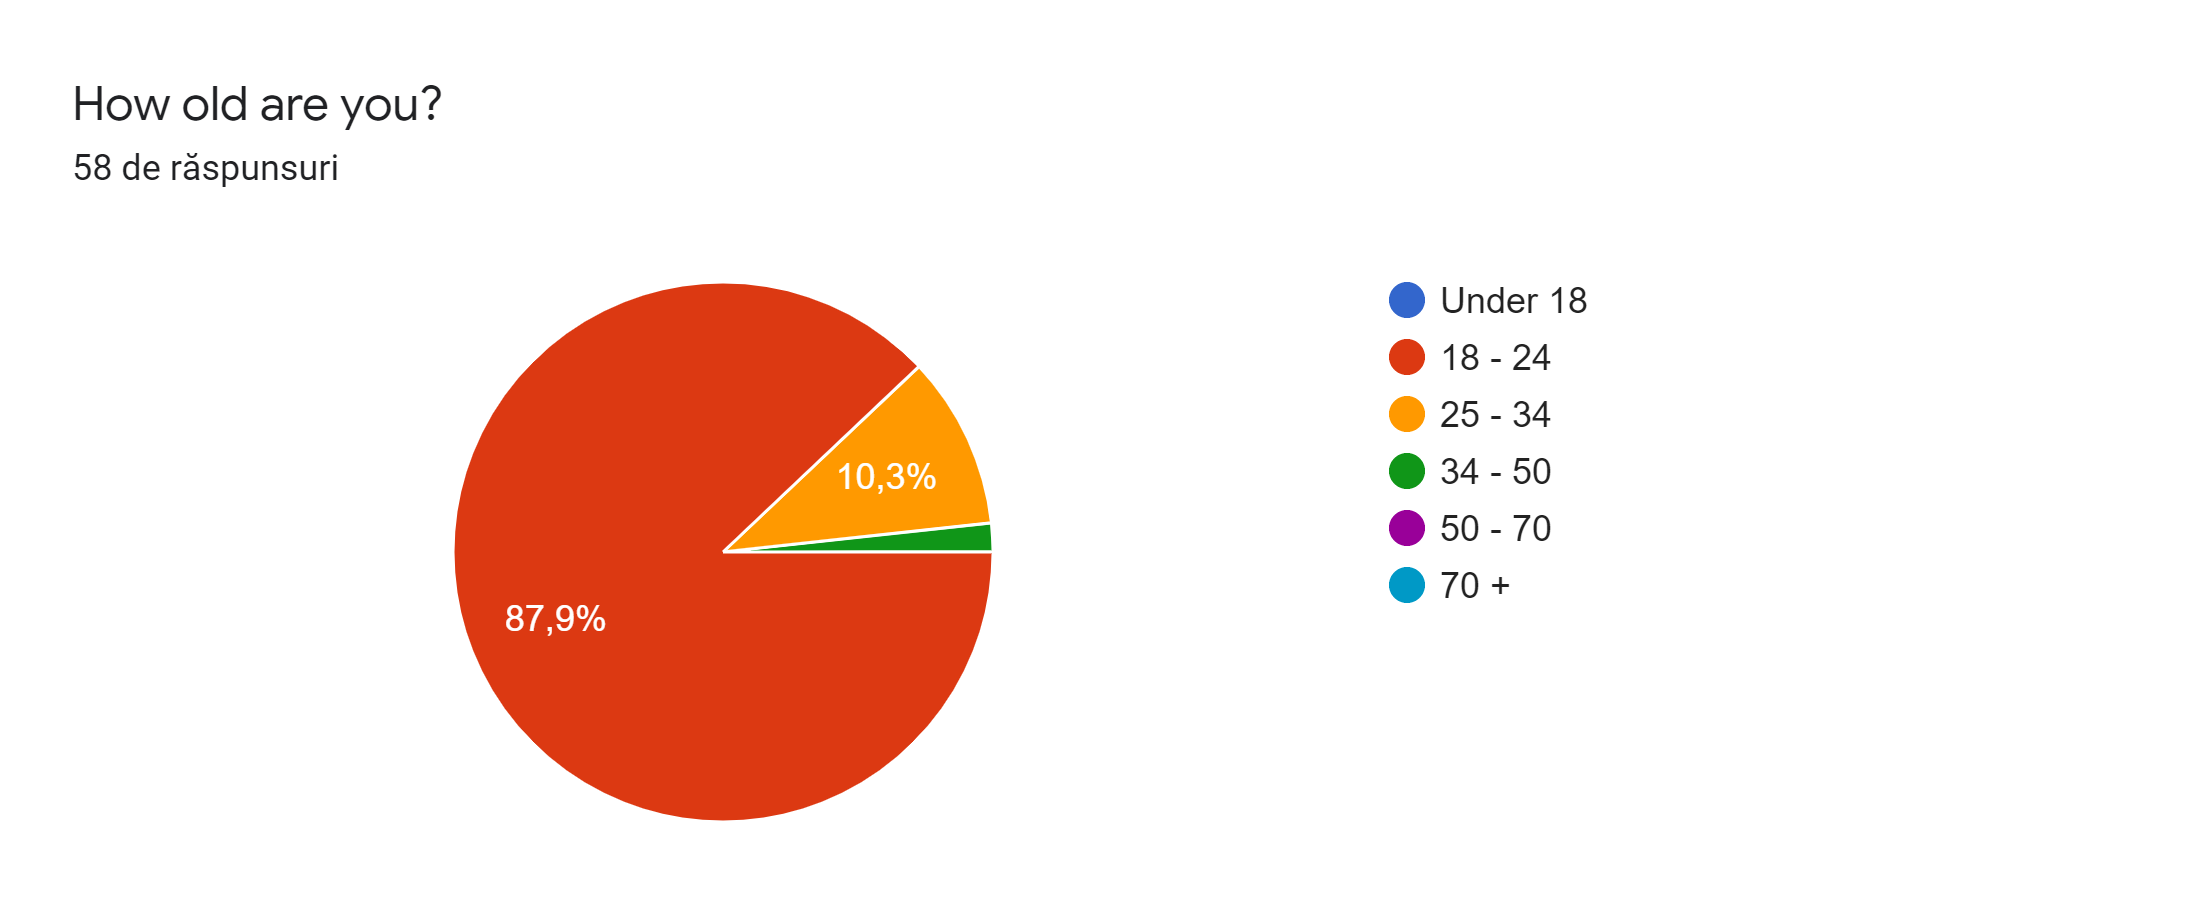
\includegraphics[width=\textwidth]{TargetGroup1}
\par
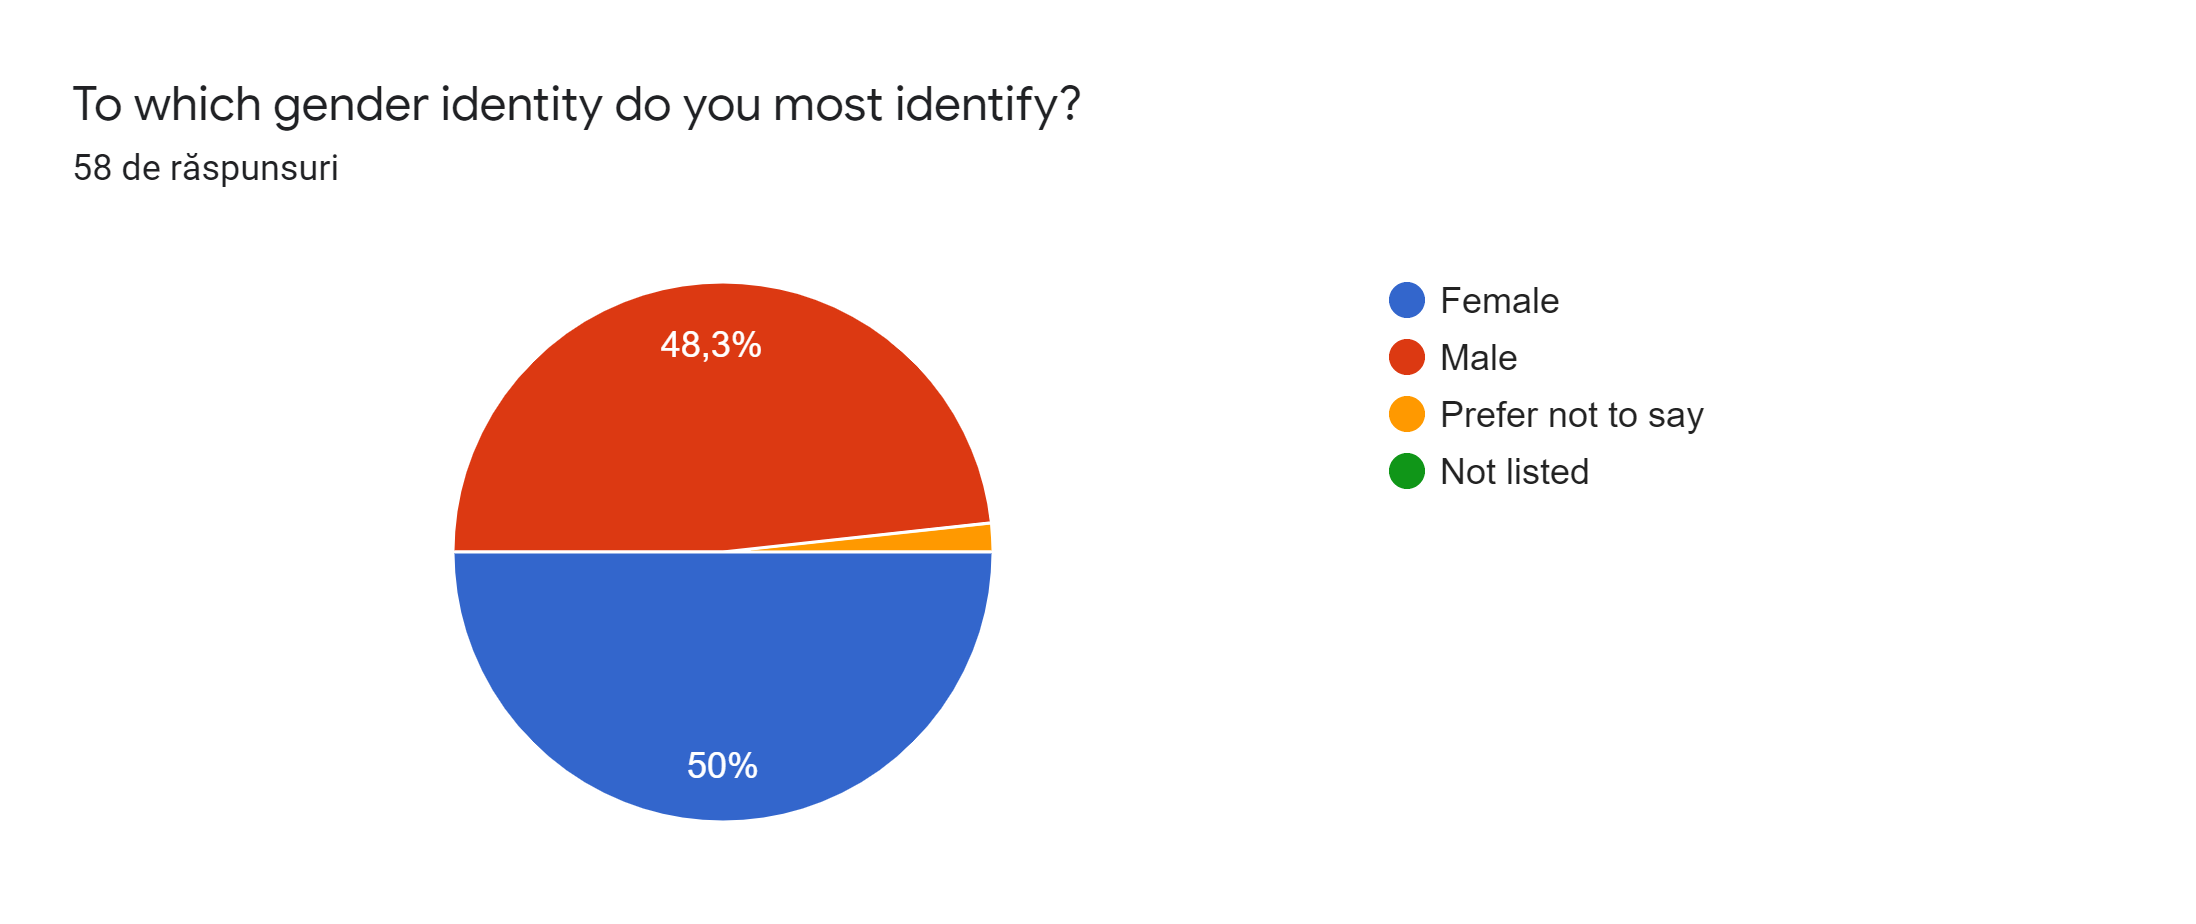
\includegraphics[width=\textwidth]{TargetGroup2}
\par The main advantage of this survey that gender majorities are in equal parts and we have a fair opinion about our product. 
\par
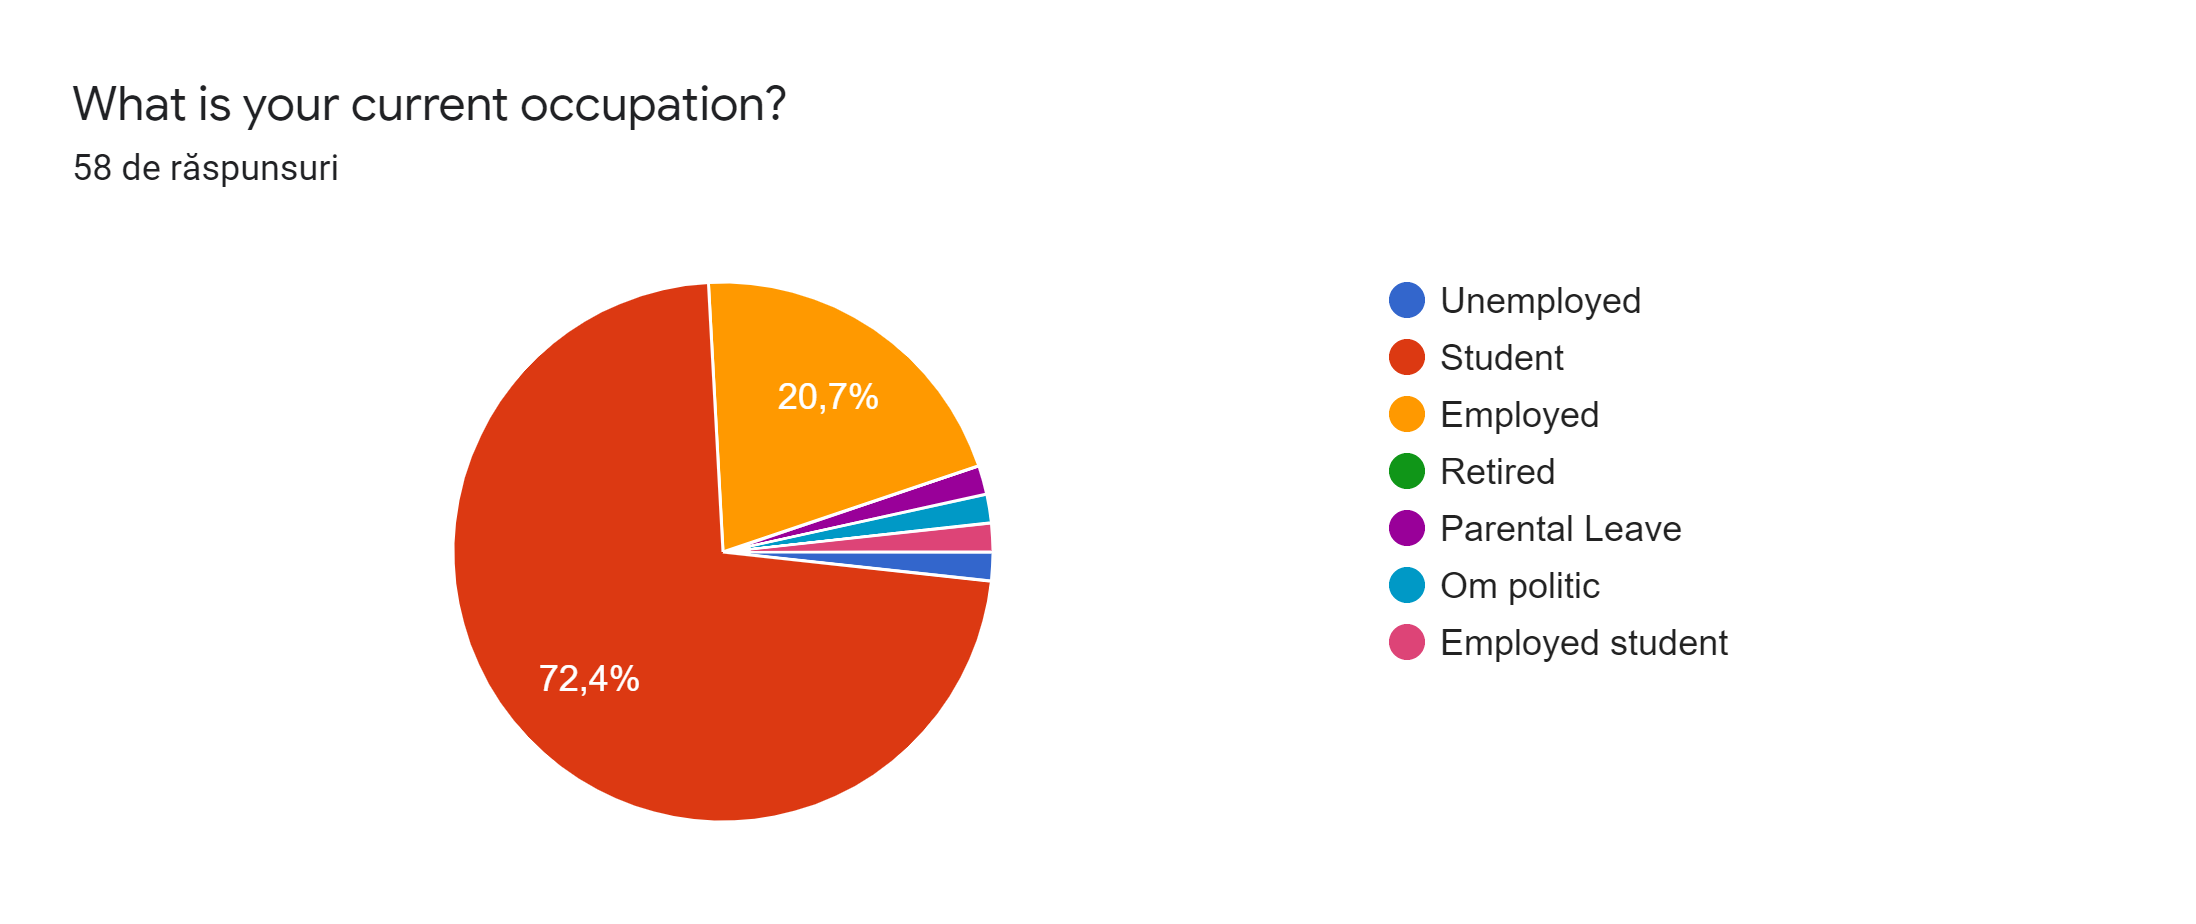
\includegraphics[width=\textwidth]{TargetGroup3}
\par Here we can see that the main parts of audience will be students and employed people. At the end of survey, we had the input line for suggestions, ideas and someone that took part in survey had written to add one more field with employed student. We thought that better will be to add ‘others’ field such that people will have more freedom to describe their current occupation. This way, we have politicians here. 
After these 3 questions we understood that the leading audience of the app will be English speaking active study-working people aged between 16 and 35 which have a lot of tasks events which are related to teams or companies that work on different platforms, or for startuppers who have an extremely flexible schedule and need a platform which will help to organize all tasks and events on one board. 


\subsection{Customer validation}
\par Another part of survey had the aim to find out if people are interested in such an app or not. Firstly, we had to find out which are their habits about organization and time management. 
\par
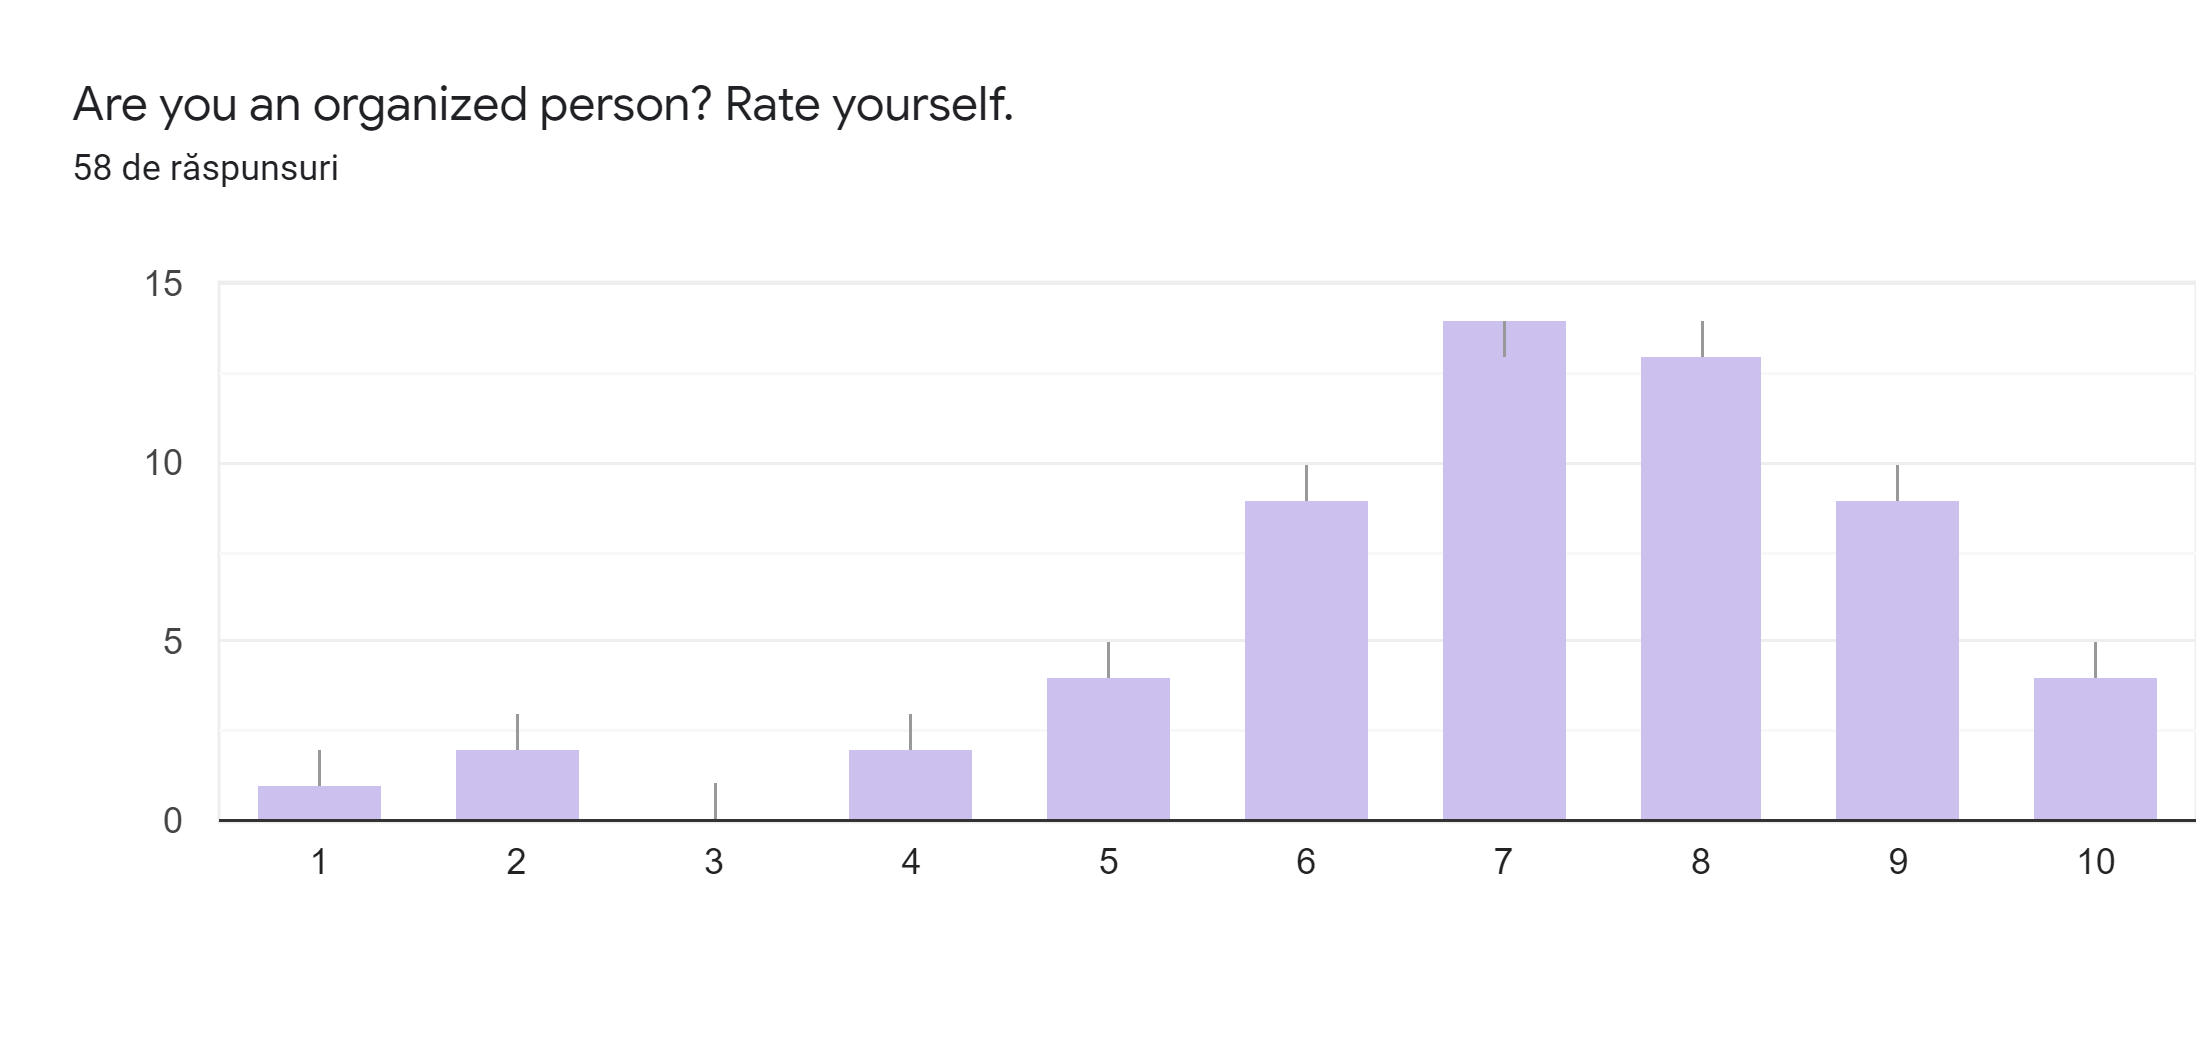
\includegraphics[width=\textwidth]{CustomerValidation1}
\par As we can see most people consider themselves moderately organized, because more than 25 people grade themselves with and 7 or 8. So we understand that people are not enough satisfied of their coordination.
\par
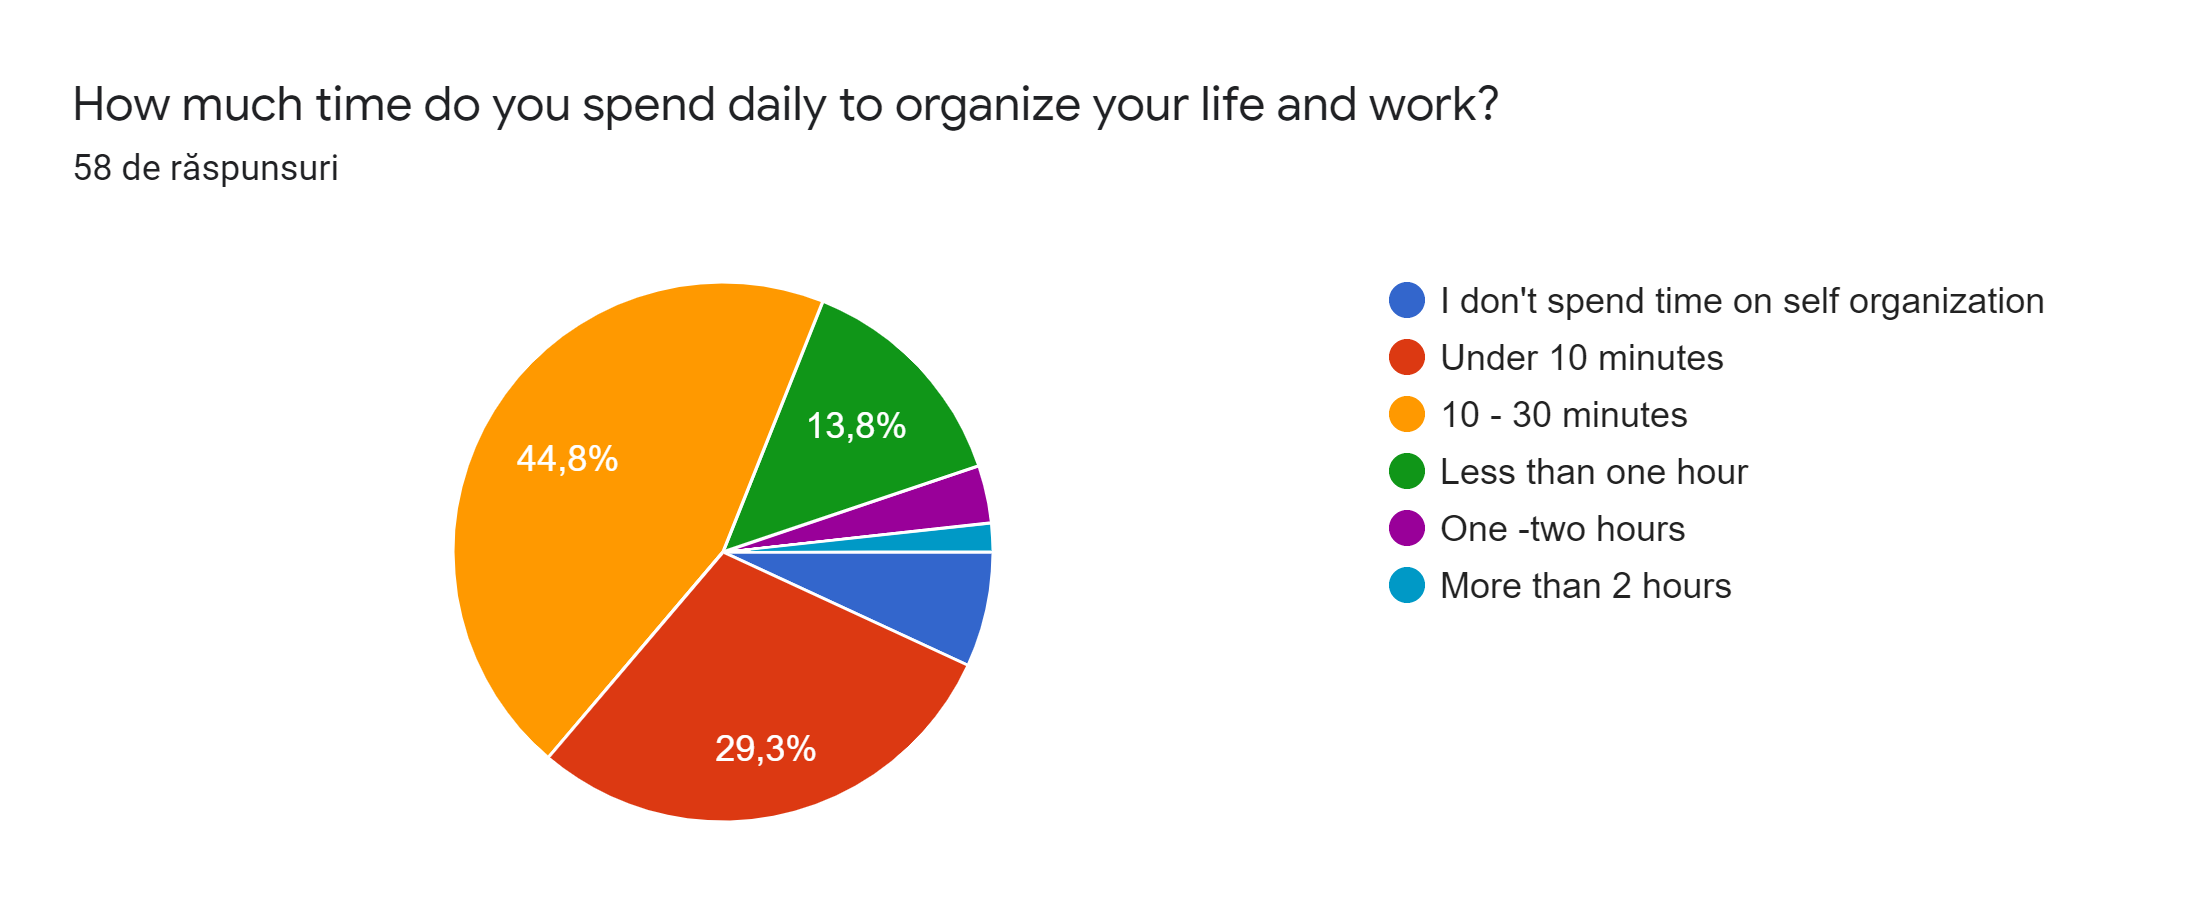
\includegraphics[width=\textwidth]{CustomerValidation2}
\par 44,8 \% of people spend 10-30 minutes per day to plan their life and work. Per year they spend 7300 minutes on this. It is 121 hours, 5 days. In their entire life they spend 250 days on arranging. There is a lot.
\par
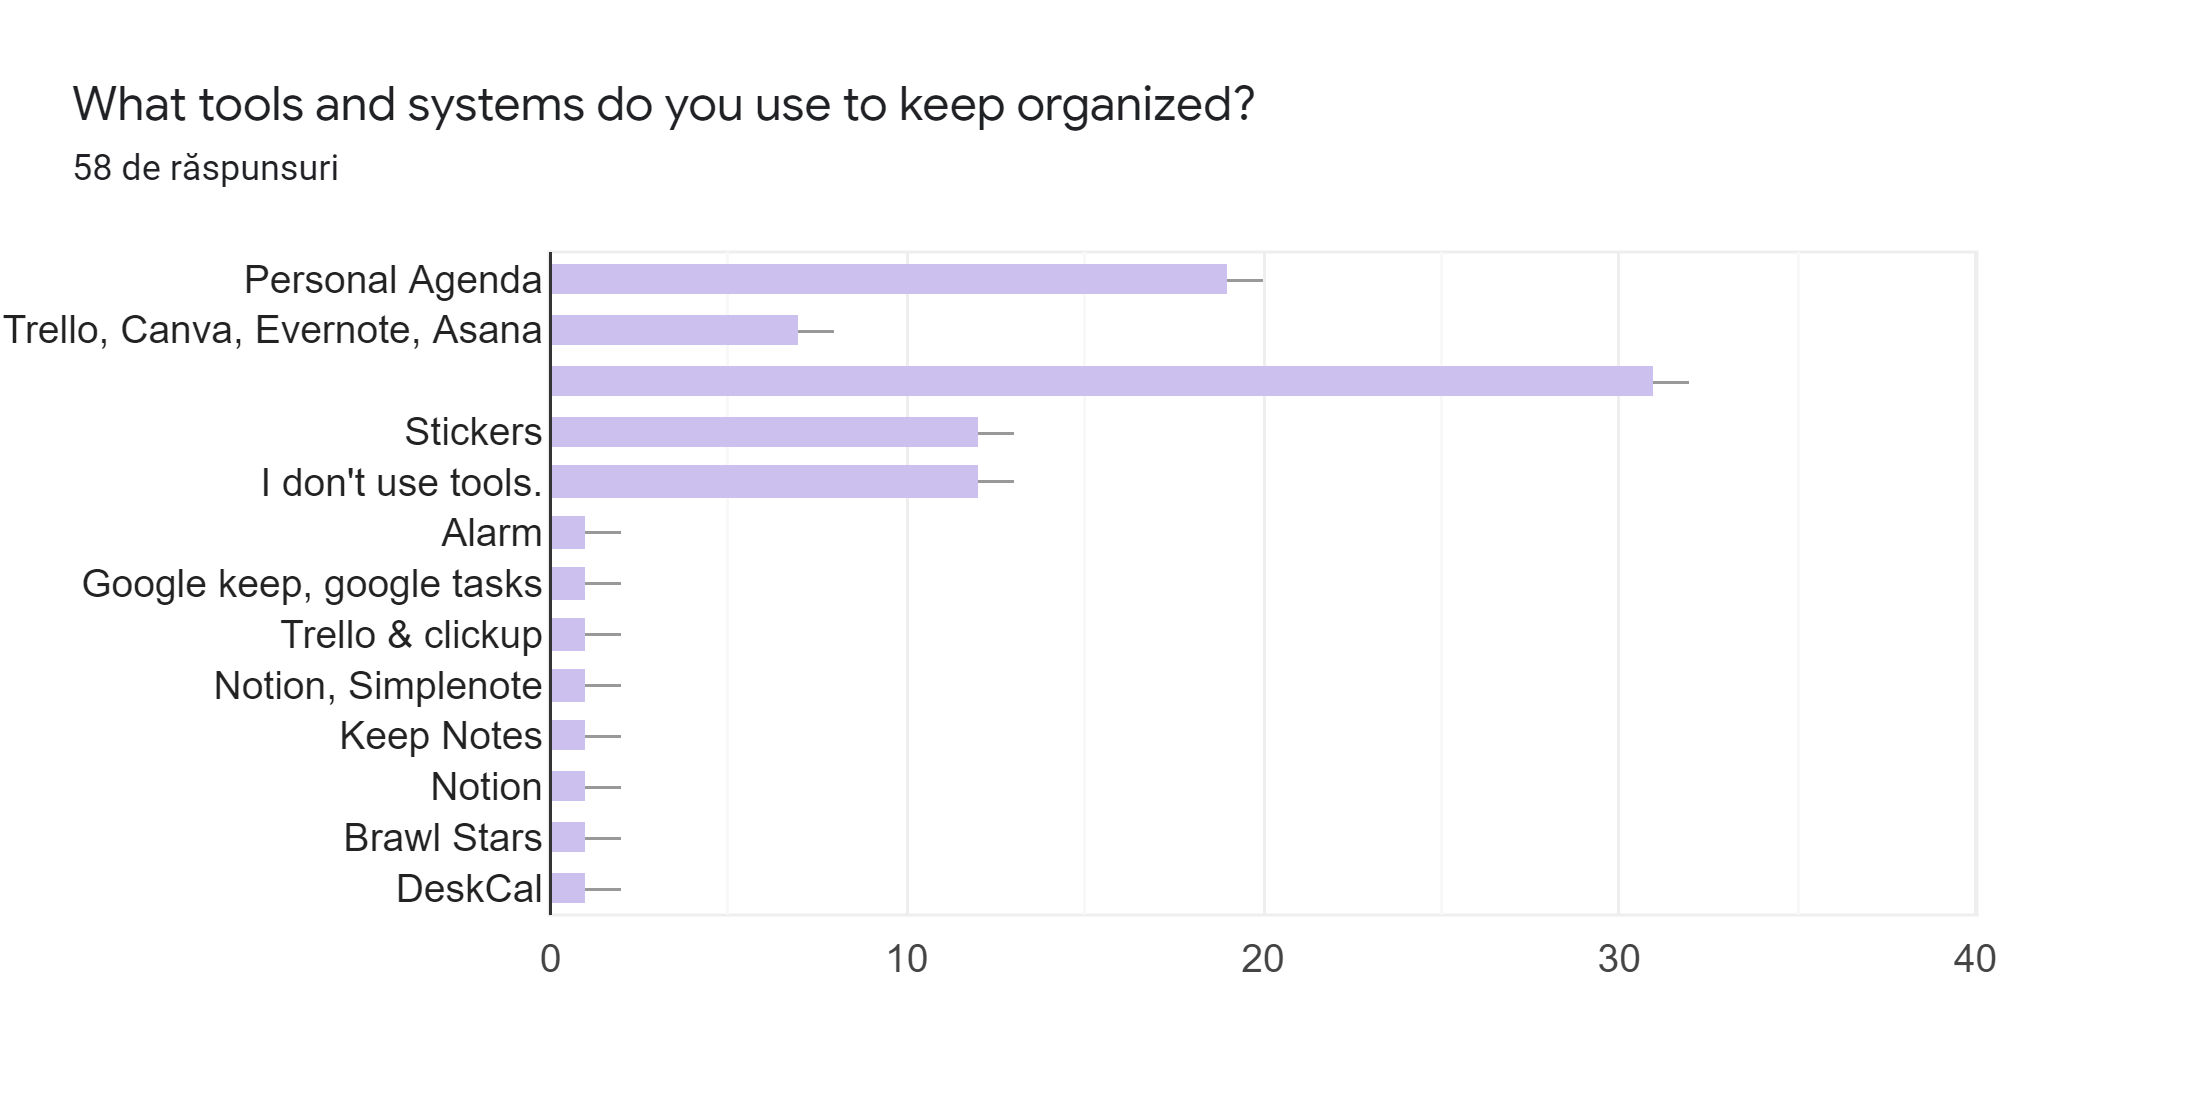
\includegraphics[width=\textwidth]{CustomerValidation3}
\par 31 humans use Google Calendar, Outlook Calendar, Todoist. This means that people like to view their task, activities, meetings in a calendar way of displaying. The second place take agendas with 19 votes. This means that even that we live in very digitalized world people choose to use the paper-based type of managing their activities and thoughts.
\par
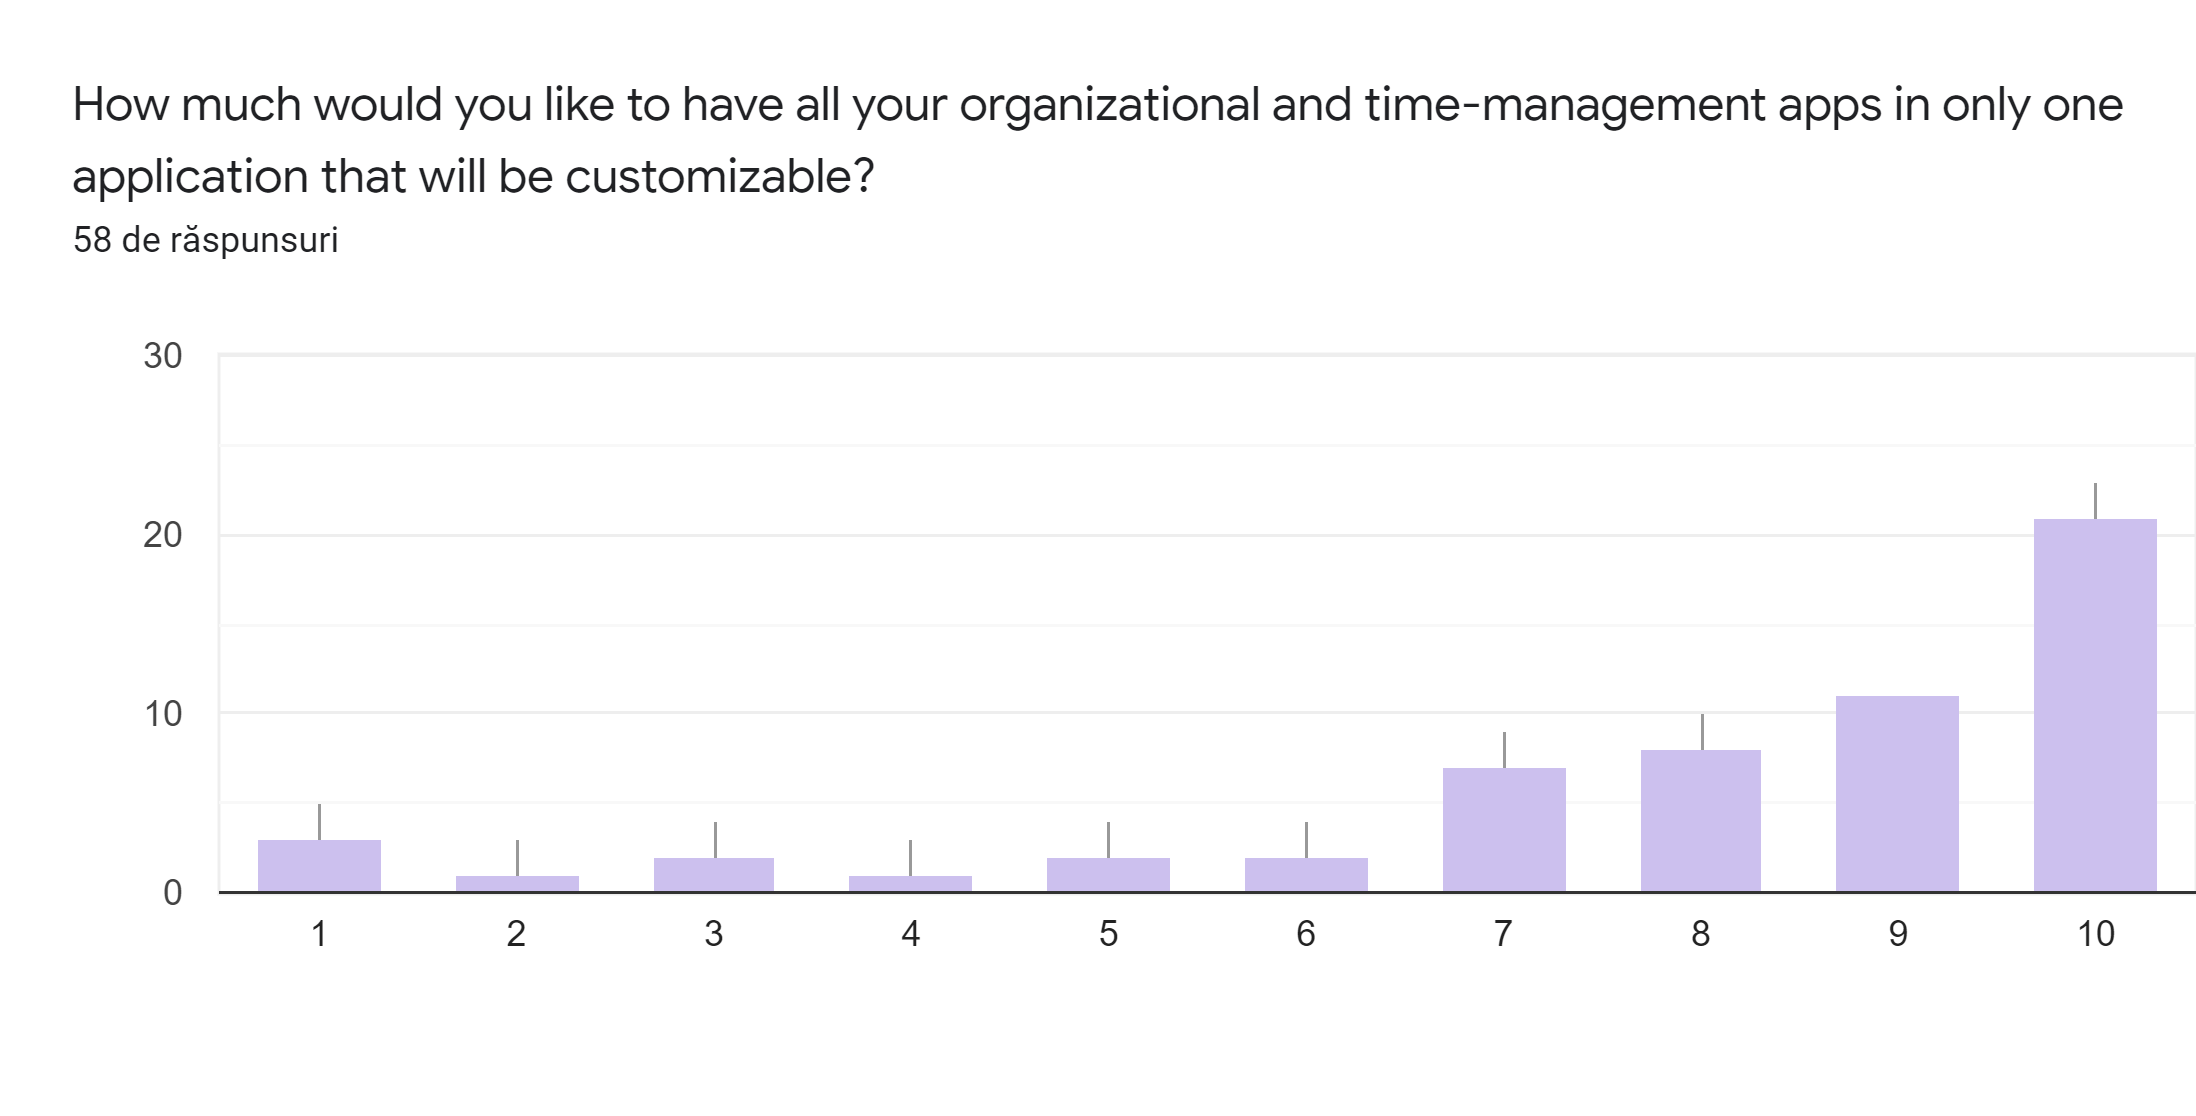
\includegraphics[width=\textwidth]{CustomerValidation4}
\par 30 assume that their desire of having an organizational and time-management app that will be customizable and will be integrated with other calendar apps is graded with 9 or 10. This is more than a half of total number of people took part and this means that the interest in such an application is highly shown. This means that developing such a concept has the right to be in production.
\par
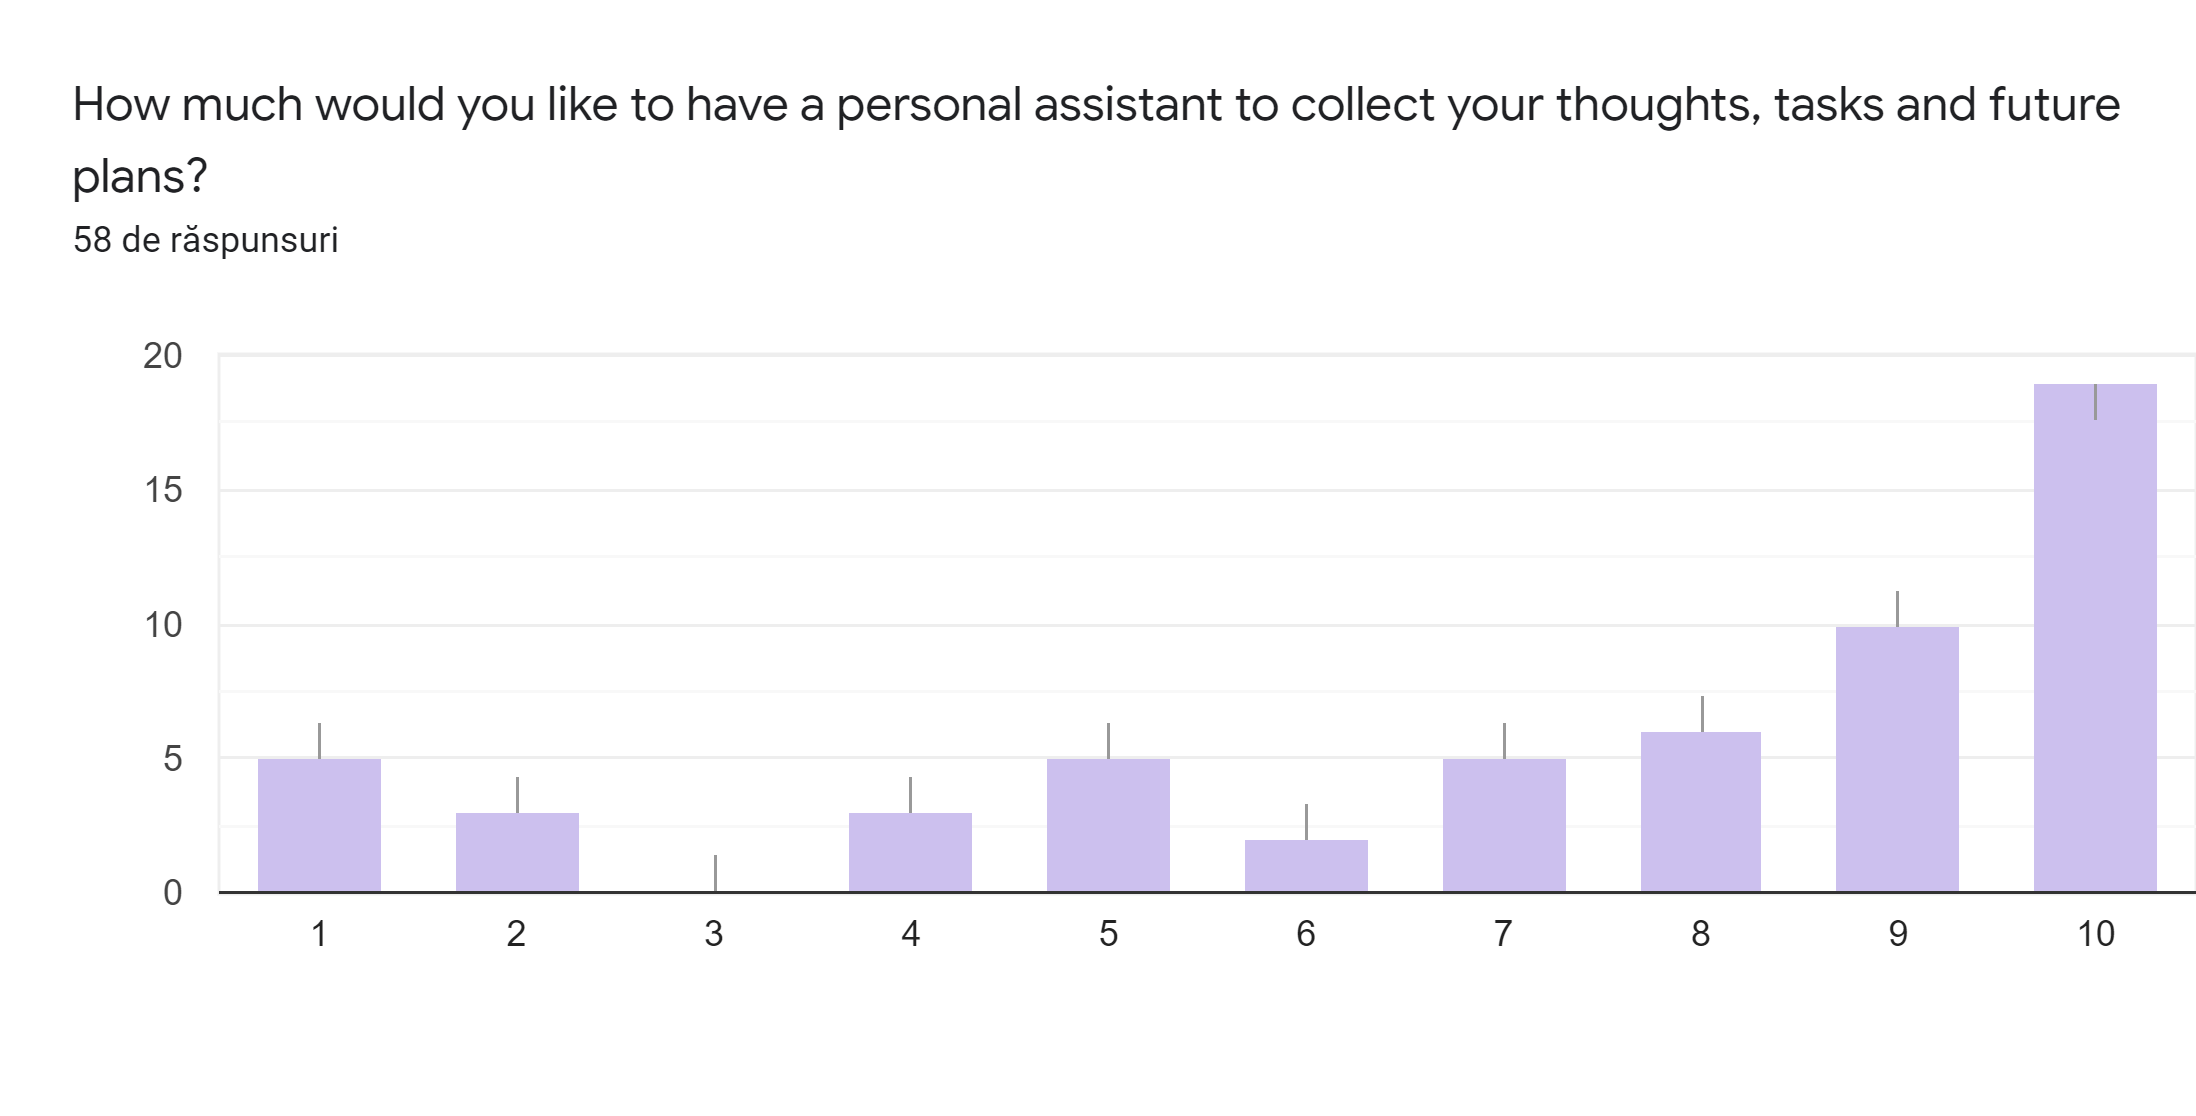
\includegraphics[width=\textwidth]{CustomerValidation5}
\par 29 people shown surely that they want to have a personal assistant to collect their thoughts, tasks and plans. It can be understood that future customers are highly interested in both of our main advantages over competitors.

\subsection{Competition}
\par 
\begin{enumerate}
	\item 	Google calendar is not the most intuitive app of using tasks and schedules it has a lot of special conditions to get the desired result 
	
	\item SuperSaaS is good at creating group schedule, but because of the design of the site is hard to understand what happens, saves the situation the support and tutorials page, it supports the work with forms directly when accessing the schedule which is very efficient in scope to get additional information  

	\item Outlook to get all the possibilities of the calendar you need to pay, is free for students and have many integrated applications which can communicate direct whit each other that increase productivity it is a combination of calendar and email it is very easy to share about events and set tasks and reminders for groups or selected people 

	\item Jorte Calendar theme changing, can use free but to get the chance to change the appearance of the calendar you need to pay subscription  

	\item Calendly it is app which works very good with establishing new meetings and events because it gave you to choose the rules that all participants can choose between the permission you establish it is time zone but the free users are limited to 1 calendar and basic functions which do not let user to feel the power of this app  
\end{enumerate}				

\clearpage